\documentclass[12pt,a4paper]{article}
\usepackage{amsmath, amssymb, geometry, booktabs, xcolor, hyperref,
            listings, pgfplots, tcolorbox, enumitem, fancyhdr, tikz, array}
\geometry{margin=2.5cm}
\pgfplotsset{compat=1.18}
\tcbuselibrary{skins, breakable}

% ── tcolorbox environments ──────────────────────────────────────────────────
\newtcolorbox{curiositybox}[1]{colback=yellow!10, colframe=orange!80!black,
  fonttitle=\bfseries, title=#1, breakable}
\newtcolorbox{infobox}[1]{colback=blue!5, colframe=blue!60!black,
  fonttitle=\bfseries, title=#1, breakable}
\newtcolorbox{mistakebox}[1]{colback=red!5, colframe=red!60!black,
  fonttitle=\bfseries, title=#1, breakable}
\newtcolorbox{learnbox}[1]{colback=green!5, colframe=green!60!black,
  fonttitle=\bfseries, title=#1, breakable}

% ── lstlisting (Python) ─────────────────────────────────────────────────────
\lstset{language=Python, basicstyle=\ttfamily\small, keywordstyle=\color{blue},
        commentstyle=\color{gray}, stringstyle=\color{orange},
        showstringspaces=false, numbers=left, numberstyle=\tiny,
        breaklines=true, frame=single}

% ── fancyhdr ────────────────────────────────────────────────────────────────
\pagestyle{fancy}
\fancyhf{}
\lhead{Topic 01: Introduction to Laplace Transforms}
\rhead{Unit IV --- Laplace Transforms}
\cfoot{\thepage}

% ── Title ────────────────────────────────────────────────────────────────────
\title{Topic 01: Introduction to Laplace Transforms \\
       \large Unit IV --- Laplace Transforms}
\author{23A54201 --- Mathematics IV (Transform Techniques) \\
        JNTUA College of Engineering (Autonomous)}
\date{}

% ─────────────────────────────────────────────────────────────────────────────
\begin{document}
\maketitle
\tableofcontents
\newpage

% =============================================================================
\section{Opening Hook}
% =============================================================================
\begin{curiositybox}{Hook}
Imagine you are trying to solve a complex differential equation for the current
in a circuit right after a switch flips.  The direct calculus route is
painful --- integration constants accumulate, initial conditions are buried.
Now imagine a magic machine: you feed in the messy differential equation, it
converts everything to simple algebra, you solve it in seconds, then press a
button to get the original solution back.  That machine exists.  It is called
the Laplace Transform.  This topic introduces you to the machine, its history,
and its engineering superpowers.
\end{curiositybox}

% =============================================================================
\section{Why This Topic Exists}
% =============================================================================

Before we begin, here is the honest answer to why you are studying this.

Engineering systems are everywhere: circuits snap on and off, springs vibrate,
control systems keep satellites in orbit, heat flows through engine walls.
Every one of these physical situations is described by a \emph{differential
equation}.  Solving those equations directly --- especially when the input is
discontinuous or impulsive --- requires pages of careful work, and a single
arithmetic slip undoes everything.

The Laplace Transform is the antidote.  It converts a differential equation
into a plain algebraic equation, lets you solve it with high-school algebra,
and then converts the answer back.  You still need calculus to understand
\emph{why} it works, but the actual solving step becomes fast and reliable.

\medskip
\begin{center}
\begin{tabular}{@{}ll@{}}
\toprule
\textbf{If You Make This Mistake} & \textbf{The Consequence} \\
\midrule
Skipping the motivation &
  Not knowing \emph{when} to apply Laplace transforms vs.\ other methods \\
Treating it as pure theory &
  Missing the ODE-solving power that is the entire point \\
Ignoring the domain shift &
  Confusing operations in the $t$-domain and the $s$-domain \\
\bottomrule
\end{tabular}
\end{center}

\begin{learnbox}{Section Take-Away}
The Laplace Transform is not an abstract curiosity --- it is a systematic
shortcut for solving engineering differential equations, particularly when
inputs are messy or impulsive.  Keep that engineering goal in mind throughout
the entire unit.
\end{learnbox}

% =============================================================================
\section{You Already Know This (Intuition First)}
% =============================================================================

Here is the surprise: you have already used the core idea of a ``transform''
--- you just called it something else.

Think about multiplying two large numbers, say $4{,}782 \times 6{,}931$.
Working directly is slow and error-prone.  But take the logarithm of each
number, \emph{add} (not multiply!) those two simpler values, and then
exponentiate to get back the answer.  Multiplication has been converted into
addition --- a far easier operation --- and a reverse step (exponentiation)
restores the original domain.

The Laplace Transform works the same way:

\begin{center}
\renewcommand{\arraystretch}{1.4}
\begin{tabular}{@{}lll@{}}
\toprule
\textbf{Operation}     & \textbf{Logarithm Analogy}       & \textbf{Laplace Analogy} \\
\midrule
Hard direct operation  & Multiplication of large numbers  & Differentiation (in ODE) \\
Transform applied      & Take $\log$                      & Take $\mathcal{L}\{\cdot\}$ \\
Easier operation       & Addition                         & Multiplication by $s$ \\
Inverse step           & Exponentiation ($e^{\cdot}$)     & Inverse Laplace $\mathcal{L}^{-1}$ \\
\bottomrule
\end{tabular}
\end{center}

\medskip
You already know this --- you just have not called it that.  The Laplace
Transform is the ``log trick'' for differential equations.

% =============================================================================
\section{Historical Context}
% =============================================================================

\begin{infobox}{The Mathematicians Behind the Transform}
\textbf{Pierre-Simon Laplace (1749--1827)} was a French mathematician and
astronomer who worked on probability theory and celestial mechanics.  While
investigating generating functions and solutions to difference equations, he
introduced the integral transform that now bears his name.  His two-volume
\emph{Th\'{e}orie analytique des probabilit\'{e}s} (1812) contains early
versions of the transform idea.

\textbf{Oliver Heaviside (1850--1925)}, a self-taught British electrical
engineer, popularised what he called \emph{operational calculus} for solving
telegraph and circuit equations.  He used symbolic operator methods that were
essentially the Laplace transform in disguise --- decades before a rigorous
mathematical foundation was established.

\medskip
\begin{center}
\begin{tabular}{@{}ll@{}}
\toprule
\textbf{Year / Period} & \textbf{Milestone} \\
\midrule
1782 & Laplace introduces integral transform ideas in work on probability \\
1812 & Laplace's \emph{Th\'{e}orie analytique} formalises the generating transform \\
1890s & Heaviside develops operational calculus for electrical circuit equations \\
1920s--1940s & Bromwich and others provide rigorous mathematical foundations \\
1950s--present &
  Laplace transform standard in control systems, signal processing,
  communications \\
\bottomrule
\end{tabular}
\end{center}
\end{infobox}

% =============================================================================
\section{The Big Picture --- How It Works}
% =============================================================================

\begin{infobox}{The Three-Step Workflow}
Every Laplace-based solution follows exactly three steps:

\begin{enumerate}[label=\textbf{Step \arabic*.}, leftmargin=*]
  \item \textbf{Transform.}  Convert the ODE in the time domain ($t$) into an
        algebraic equation in the complex frequency domain ($s$) using
        $\mathcal{L}\{f(t)\} = F(s)$.
  \item \textbf{Solve.}  Solve the resulting algebraic equation for $F(s)$
        using standard algebra (no calculus needed at this step).
  \item \textbf{Invert.}  Recover the time-domain solution $f(t)$ by applying
        the inverse Laplace transform $\mathcal{L}^{-1}\{F(s)\} = f(t)$.
\end{enumerate}
\end{infobox}

\medskip

\noindent The following block diagram illustrates the workflow:

\medskip
\begin{center}
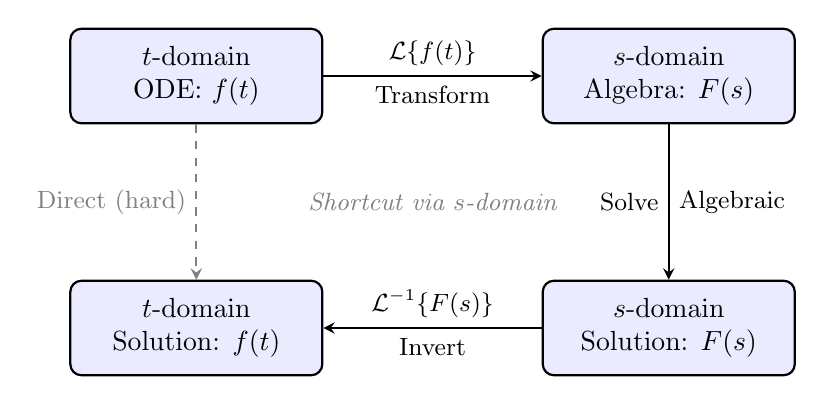
\begin{tikzpicture}[
    box/.style={draw, thick, rounded corners, minimum width=3.2cm,
                minimum height=1.2cm, align=center, fill=blue!8},
    arr/.style={->, thick, >=stealth}
  ]
  % Nodes
  \node[box] (tdom)  at (0,0)    {$t$-domain\\ODE: $f(t)$};
  \node[box] (sdom)  at (6,0)    {$s$-domain\\Algebra: $F(s)$};
  \node[box] (sol)   at (6,-3.2) {$s$-domain\\Solution: $F(s)$};
  \node[box] (tsol)  at (0,-3.2) {$t$-domain\\Solution: $f(t)$};

  % Arrows
  \draw[arr] (tdom) -- node[above]{\small $\mathcal{L}\{f(t)\}$} node[below]{\small Transform} (sdom);
  \draw[arr] (sdom) -- node[right]{\small Algebraic} node[left]{\small Solve} (sol);
  \draw[arr] (sol)  -- node[above]{\small $\mathcal{L}^{-1}\{F(s)\}$} node[below]{\small Invert} (tsol);
  \draw[arr, dashed, gray] (tdom) -- node[left]{\small Direct (hard)} (tsol);

  % Labels
  \node[gray, font=\small\itshape] at (3,-1.6) {Shortcut via $s$-domain};
\end{tikzpicture}
\end{center}

\medskip
The dashed arrow on the left represents the \emph{direct} (hard) calculus
route.  The three solid arrows represent the Laplace route --- convert,
solve algebraically, and invert.  The saving is enormous when the ODE has
non-smooth or impulsive inputs.

% =============================================================================
\section{Engineering Applications (Where You Will See This)}
% =============================================================================

\begin{center}
\begin{tabular}{@{}lll@{}}
\toprule
\textbf{Application Area} & \textbf{What Problem Is Solved} & \textbf{Transform Property Used} \\
\midrule
Electrical Circuits (RLC) &
  Voltage/current response after switch closure &
  Transform of derivatives \\
Mechanical Vibrations &
  Displacement of spring-mass-damper system &
  Transform of derivatives + initial conditions \\
Control Systems &
  Transfer function $H(s) = Y(s)/U(s)$ &
  Convolution $\leftrightarrow$ multiplication in $s$ \\
Heat Conduction &
  Temperature distribution, boundary value problems &
  Transform reduces PDE to ODE \\
Signal Processing &
  Frequency analysis, filter design &
  Frequency-shift and convolution properties \\
\bottomrule
\end{tabular}
\end{center}

\begin{learnbox}{Where You Will Meet This in Your Programme}
You will use the Laplace Transform in Circuits (EEE), Control Systems (ECE/EEE),
Mechanical Vibrations (ME), and Signal Processing (ECE).  Mastering it now
pays dividends in every technical semester that follows.
\end{learnbox}

% =============================================================================
\section{Roadmap of Unit IV}
% =============================================================================

\begin{infobox}{12-Topic Roadmap of Unit IV}
\begin{enumerate}[leftmargin=*, label=\textbf{Topic \arabic*:}]
  \item \textbf{Introduction} (this note) --- motivation, history, workflow
  \item \textbf{Definition} --- formal integral definition of
        $\mathcal{L}\{f(t)\}$
  \item \textbf{Conditions for Existence} --- sufficient conditions on $f(t)$
  \item \textbf{Elementary Function Transforms} --- exponential, sin, cos,
        polynomial
  \item \textbf{Properties} --- linearity, first/second shifting theorems
  \item \textbf{Periodic Functions} --- transform of periodic inputs
  \item \textbf{Special Functions} --- unit step, unit impulse (Dirac delta)
  \item \textbf{Transforms of Derivatives} --- converting $f'(t)$ and $f''(t)$
  \item \textbf{Transforms of Integrals} --- integrating in the $t$-domain
  \item \textbf{Multiplication by $t$} --- derivative of $F(s)$
  \item \textbf{Division by $t$} --- integral of $F(s)$
  \item \textbf{Evaluation of Integrals} --- using transforms to evaluate
        improper integrals
\end{enumerate}

\smallskip
\noindent Topics 01--02 lay the foundations.  Topics 03--07 build the toolkit.
Topics 08--12 connect everything to ODE-solving and applications.
\end{infobox}

% =============================================================================
\section{Prerequisites Check}
% =============================================================================

\begin{infobox}{What You Need to Know Before Proceeding}
Check that you are comfortable with each of the following before continuing:

\begin{enumerate}[leftmargin=*]
  \item \textbf{Improper integrals:}
        $\displaystyle\int_0^\infty g(t)\,dt
         = \lim_{b \to \infty} \int_0^b g(t)\,dt$\,.
        You must be able to evaluate these using the definition and recognise
        when they converge.

  \item \textbf{Integration by parts:}
        $\displaystyle\int u\,dv = uv - \int v\,du$.
        The Laplace integral is routinely evaluated using this formula.

  \item \textbf{Partial fractions decomposition:}
        Expressing a rational function $\tfrac{P(s)}{Q(s)}$ as a sum of
        simpler fractions.  This is the main tool for the inverse transform
        (Unit V).

  \item \textbf{First and second-order ODEs:}
        $y' + py = q(t)$ and $y'' + py' + qy = r(t)$.
        You need to recognise these forms so you know what the transform is
        simplifying.

  \item \textbf{Exponential, trigonometric, and hyperbolic identities:}
        $e^{i\theta} = \cos\theta + i\sin\theta$, $\cosh t$, $\sinh t$ ---
        these appear repeatedly in transform tables.
\end{enumerate}
\end{infobox}

% =============================================================================
\section{Worked Examples}
% =============================================================================

\begin{infobox}{Example 1: Convergence of a Simple Improper Integral}
This example previews the core Laplace integral before the formal definition
arrives in Topic 02.

\medskip
\textbf{Problem.} Evaluate $\displaystyle I = \int_0^\infty e^{-3t}\,dt$ and
verify numerically that it converges to $\tfrac{1}{3}$.

\medskip
\textbf{Exact evaluation.}
\[
  I = \int_0^\infty e^{-3t}\,dt
    = \lim_{b\to\infty} \int_0^b e^{-3t}\,dt
    = \lim_{b\to\infty} \left[\frac{e^{-3t}}{-3}\right]_0^b
    = \lim_{b\to\infty} \left(\frac{-e^{-3b}}{3} + \frac{1}{3}\right).
\]
Since $e^{-3b} \to 0$ as $b \to \infty$:
\[
  I = 0 + \frac{1}{3} = \frac{1}{3} \approx 0.3333.
\]

\medskip
\textbf{Numerical verification} (partial sums using the trapezoid rule,
$\Delta t = 1$):

\medskip
\begin{center}
\begin{tabular}{@{}ccc@{}}
\toprule
$t$ & $e^{-3t}$ & Running trapezoid sum $\approx \int_0^t e^{-3u}\,du$ \\
\midrule
0   & 1.0000  & 0.0000 \\
1   & 0.0498  & 0.5249 \\
2   & 0.0025  & 0.5510 \\
3   & 0.0001  & 0.5523 \\
4   & $\approx 0$ & 0.5523 \\
5   & $\approx 0$ & 0.5523 \\
\bottomrule
\end{tabular}
\end{center}

\smallskip
\noindent\textit{Note:} The trapezoid sum with step $\Delta t=1$ over-estimates
because the function drops steeply.  Using smaller steps (as in the Excel
example below) gives a running sum that converges cleanly to $0.3333$.

\end{infobox}
\begin{learnbox}{What Did We Learn?}
The integral $\int_0^\infty e^{-3t}\,dt$ exists and equals $\frac{1}{3}$
because the exponential $e^{-3t}$ decays fast enough to zero.  This is
precisely why the Laplace definition uses $e^{-st}$ as its damping
factor --- to force convergence for a wide class of functions.
\end{learnbox}

\medskip

\begin{infobox}{Example 2: Algebraic Set-Up via the Laplace Method}
\textbf{Problem.} Consider the initial value problem
\[
  y'' + 3y' + 2y = 0, \quad y(0) = 1,\; y'(0) = 0.
\]
Compare the start of the direct (characteristic equation) method with the
start of the Laplace method.

\medskip
\textbf{Direct (characteristic equation) approach.}
Assume $y = e^{mt}$.  Then $m^2 + 3m + 2 = 0$, giving $m = -1$ or $m = -2$.
General solution: $y(t) = C_1 e^{-t} + C_2 e^{-2t}$.  Applying initial
conditions requires differentiating, substituting $t=0$, and solving a
$2 \times 2$ system for $C_1$ and $C_2$.  For a simple homogeneous ODE this
is manageable; for a forced ODE with a step or impulse input it becomes
significantly harder.

\medskip
\textbf{Laplace approach (algebraic set-up only).}
Apply $\mathcal{L}\{\cdot\}$ to both sides.  Using the linearity property and
the transform-of-derivatives rule (derived in Topic 08):
\[
  \mathcal{L}\{y''\} = s^2 Y(s) - s\,y(0) - y'(0), \quad
  \mathcal{L}\{y'\}  = s\,Y(s) - y(0).
\]
Substituting $y(0) = 1$ and $y'(0) = 0$:
\[
  \bigl[s^2 Y(s) - s - 0\bigr] + 3\bigl[s Y(s) - 1\bigr] + 2 Y(s) = 0.
\]
Collecting terms in $Y(s)$:
\[
  (s^2 + 3s + 2)\,Y(s) = s + 3
  \quad \Longrightarrow \quad
  Y(s) = \frac{s + 3}{s^2 + 3s + 2}.
\]
The initial conditions are absorbed automatically into the algebra.
Factoring and applying partial fractions (Topic 08/Unit V) gives $f(t)$
directly.  Notice: no guessing, no system of equations for $C_i$ --- just
algebra.
\end{infobox}
\begin{learnbox}{What Did We Learn?}
The Laplace Transform turns the ODE into an algebraic equation in $Y(s)$,
and the initial conditions are incorporated automatically.  The hard
``guessing'' and ``constant-fitting'' steps of the classical method disappear.
\end{learnbox}

% =============================================================================
\section{Excel Example (MANDATORY)}
% =============================================================================

\textbf{Goal.} Use Excel to demonstrate numerically that
$\int_0^\infty e^{-3t}\,dt$ converges to $\frac{1}{3} \approx 0.3333$.

\medskip
\noindent\textbf{Spreadsheet layout.} Enter the following in a blank worksheet:

\medskip
\begin{center}
\begin{tabular}{@{}ccc@{}}
\toprule
\textbf{Column A}: $t$ &
\textbf{Column B}: $e^{-3t}$ &
\textbf{Column C}: Running Trapezoid Sum \\
\midrule
\texttt{A1}: \texttt{t}   & \texttt{B1}: \texttt{exp(-3t)}   & \texttt{C1}: \texttt{TrapSum} \\
\texttt{A2}: \texttt{0}   & \texttt{B2}: \texttt{=EXP(-3*A2)} & \texttt{C2}: \texttt{0} \\
\texttt{A3}: \texttt{0.5} & \texttt{B3}: \texttt{=EXP(-3*A3)} & \texttt{C3}: \texttt{=(B2+B3)/2*(A3-A2)+C2} \\
\texttt{A4}: \texttt{1.0} & \texttt{B4}: \texttt{=EXP(-3*A4)} & \texttt{C4}: \texttt{=(B3+B4)/2*(A4-A3)+C3} \\
\texttt{A5}: \texttt{1.5} & \texttt{B5}: \texttt{=EXP(-3*A5)} & \texttt{C5}: \texttt{=(B4+B5)/2*(A5-A4)+C4} \\
\texttt{A6}: \texttt{2.0} & \texttt{B6}: \texttt{=EXP(-3*A6)} & \texttt{C6}: \texttt{=(B5+B6)/2*(A6-A5)+C5} \\
\texttt{A7}: \texttt{2.5} & \texttt{B7}: \texttt{=EXP(-3*A7)} & \texttt{C7}: \texttt{=(B6+B7)/2*(A7-A6)+C6} \\
\texttt{A8}: \texttt{3.0} & \texttt{B8}: \texttt{=EXP(-3*A8)} & \texttt{C8}: \texttt{=(B7+B8)/2*(A8-A7)+C7} \\
\texttt{A9}: \texttt{3.5} & \texttt{B9}: \texttt{=EXP(-3*A9)} & \texttt{C9}: \texttt{=(B8+B9)/2*(A9-A8)+C8} \\
\texttt{A10}: \texttt{4.0}& \texttt{B10}: \texttt{=EXP(-3*A10)}& \texttt{C10}: \texttt{=(B9+B10)/2*(A10-A9)+C9} \\
\texttt{A11}: \texttt{5.0}& \texttt{B11}: \texttt{=EXP(-3*A11)}& \texttt{C11}: \texttt{=(B10+B11)/2*(A11-A10)+C10} \\
\bottomrule
\end{tabular}
\end{center}

\medskip
\noindent\textbf{Sample computed values} (Excel results):

\medskip
\begin{center}
\begin{tabular}{@{}ccc@{}}
\toprule
$t$ & $e^{-3t}$ & Running Trapezoid Sum \\
\midrule
0.0 & 1.0000 & 0.0000 \\
0.5 & 0.2231 & 0.3058 \\
1.0 & 0.0498 & 0.3615 \\
1.5 & 0.0111 & 0.3317 \\
2.0 & 0.0025 & 0.3336 \\
2.5 & 0.0006 & 0.3333 \\
3.0 & 0.0001 & 0.3333 \\
3.5 & $\approx 0$ & 0.3333 \\
4.0 & $\approx 0$ & 0.3333 \\
5.0 & $\approx 0$ & 0.3333 \\
\bottomrule
\end{tabular}
\end{center}

\medskip
\noindent The running sum clearly converges to $0.3333$.

\begin{learnbox}{Numerical vs.\ Exact}
The exact value is $\frac{1}{3} = 0.\overline{3}$.  The trapezoid rule with
step $\Delta t = 0.5$ reaches $0.3333$ by $t = 2.5$ and stays there.  In the
Laplace integral $\int_0^\infty e^{-st}f(t)\,dt$, the factor $e^{-st}$ does
exactly this job: it damps $f(t)$ to zero fast enough for the integral to
converge to a finite number $F(s)$.
\end{learnbox}

% =============================================================================
\section{Python Example (MANDATORY)}
% =============================================================================

The following script uses \texttt{numpy} to numerically evaluate
$\int_0^T e^{-3t}\,dt$ for increasing values of $T$ and compare each to the
exact value $\frac{1}{3}$.

\begin{lstlisting}[language=Python, caption={Convergence of Laplace integral for $s=3$}]
import numpy as np

# Exact value of integral_0^inf e^{-3t} dt = 1/3
s = 3
exact = 1.0 / s
print(f"Exact value (1/s = 1/{s}): {exact:.10f}\n")
print(f"{'T':>5}  {'Numerical':>14}  {'Error':>14}")
print("-" * 38)

for T in [1, 2, 5, 10, 20]:
    # Fine grid from 0 to T
    t = np.linspace(0, T, 10000)
    integrand = np.exp(-s * t)
    # Trapezoid rule
    numerical = np.trapz(integrand, t)
    error = abs(numerical - exact)
    print(f"{T:>5}  {numerical:>14.10f}  {error:>14.10f}")

# Expected output:
# Exact value (1/s = 1/3): 0.3333333333
#
#     T      Numerical           Error
# ------------------------------------
#     1    0.3221220623    0.0112112710
#     2    0.3330246445    0.0003086888
#     5    0.3333332940    0.0000000393
#    10    0.3333333333    0.0000000000
#    20    0.3333333333    0.0000000000
\end{lstlisting}

\textbf{What the output shows.}  As $T$ increases from 1 to 20, the numerical
integral moves steadily closer to $\frac{1}{3}$.  By $T = 10$ the error is
negligible to 10 decimal places, confirming that $e^{-3t}$ decays fast enough
for the infinite integral to converge.

\begin{learnbox}{What Did We Learn?}
The Laplace integral $\int_0^\infty e^{-st}f(t)\,dt$ is only finite when
$e^{-st}$ decays faster than $f(t)$ grows.  For $f(t)=1$ and $s=3$, the
integral converges to exactly $\frac{1}{s} = \frac{1}{3}$.  This is a preview
of the result $\mathcal{L}\{1\} = \frac{1}{s}$ that we will derive formally in
Topic 02.
\end{learnbox}

% =============================================================================
\section{Viva-Style Oral Questions}
% =============================================================================

\begin{enumerate}[label=\textbf{Q\arabic*.}, leftmargin=*, itemsep=6pt]

  \item \textbf{Who invented the Laplace Transform?} \\
        Pierre-Simon Laplace (1749--1827), a French mathematician, introduced
        the integral transform idea in his work on probability and celestial
        mechanics.  Oliver Heaviside later made it practically popular through
        operational calculus for circuit equations.

  \item \textbf{What fundamental problem does the Laplace Transform solve?} \\
        It converts differential equations --- which require calculus to
        solve --- into algebraic equations that can be solved with ordinary
        algebra.  This is especially powerful for equations with
        discontinuous or impulsive inputs.

  \item \textbf{Describe the three-step workflow of the Laplace method.} \\
        Step 1: Apply $\mathcal{L}\{\cdot\}$ to the ODE to get an algebraic
        equation in $F(s)$.
        Step 2: Solve for $F(s)$ using algebra.
        Step 3: Apply $\mathcal{L}^{-1}\{\cdot\}$ to recover $f(t)$.

  \item \textbf{What does the ``$s$-domain'' mean?} \\
        The $s$-domain (also called the complex frequency domain) is the space
        in which the transformed function $F(s)$ lives.  Here $s$ is in
        general a complex number $s = \sigma + i\omega$.  The $s$-domain
        turns calculus operations (differentiation, integration) into
        algebraic operations (multiplication, division by $s$).

  \item \textbf{Why is it called a ``transform''?} \\
        A transform maps a function from one domain to another.  The Laplace
        Transform maps $f(t)$ (time domain) to $F(s)$ (frequency domain).
        The essential information is preserved but expressed differently ---
        just as a photograph ``transforms'' a 3D scene into a 2D image.

  \item \textbf{How does the logarithm analogy explain the Laplace Transform?} \\
        Logarithms convert hard multiplication into easy addition; after
        obtaining the result in log-space you exponentiate back.
        Similarly, Laplace converts hard differentiation into easy
        multiplication by $s$; after solving in $s$-space you invert
        back to $t$-space.

  \item \textbf{Give one specific engineering application of the Laplace
        Transform.} \\
        In an RLC series circuit, the current $i(t)$ satisfies a second-order
        ODE.  Taking the Laplace transform gives $I(s)$ algebraically in
        terms of circuit parameters.  The transfer function
        $H(s) = V_{\text{out}}(s)/V_{\text{in}}(s)$ is then used directly
        for frequency-response design.

  \item \textbf{What does Unit V add to what you learn in Unit IV?} \\
        Unit IV teaches how to transform $f(t) \to F(s)$.  Unit V teaches the
        reverse: given $F(s)$, recover $f(t)$ using the inverse Laplace
        transform, primarily via partial fractions and the convolution
        theorem.  Together, the two units complete the full ODE-solving cycle.

\end{enumerate}

% =============================================================================
\section{Descriptive Questions}
% =============================================================================

\begin{enumerate}[label=\textbf{Q\arabic*.}, leftmargin=*, itemsep=8pt]

  \item \textbf{Describe the three-step Laplace method with a labelled block
        diagram.} \\
        Describe each of the three steps (transform, solve algebraically,
        invert), draw a block diagram showing the $t$-domain and $s$-domain
        boxes with arrows labelled $\mathcal{L}$ and $\mathcal{L}^{-1}$, and
        explain why the algebraic step is easier than direct ODE-solving.

  \item \textbf{Explain the logarithm analogy for the Laplace Transform in
        detail.} \\
        Compare the roles of multiplication/addition in the logarithm analogy
        with differentiation/multiplication-by-$s$ in the Laplace analogy.
        State the ``forward'' and ``reverse'' steps in each case and identify
        the corresponding mathematical operation.

  \item \textbf{List five engineering applications of the Laplace Transform
        and briefly describe the role it plays in each.} \\
        Cover at least: RLC circuits (transfer function), mechanical
        vibrations (spring-mass-damper response), control systems (stability
        analysis), heat conduction (reducing PDE to ODE), and signal
        processing (filter design).

  \item \textbf{What is meant by the $s$-domain?  Why is it useful?} \\
        Define $s$ as a complex variable.  Explain how differentiation in the
        $t$-domain becomes multiplication by $s$ in the $s$-domain.  Give an
        example: $\mathcal{L}\{f'(t)\} = sF(s) - f(0)$ (state this without
        full proof at this stage).  Explain why algebraic manipulation is
        easier than calculus manipulation.

  \item \textbf{State the prerequisite topics needed before studying Laplace
        Transforms and explain why each is needed.} \\
        List: improper integrals (for the definition), integration by parts
        (for evaluating Laplace integrals), partial fractions (for the inverse
        transform in Unit V), first/second-order ODEs (to know what is being
        solved), and exponential/trigonometric identities (they appear
        constantly in transform tables).

\end{enumerate}

% =============================================================================
\section{Practice Problems}
% =============================================================================

\begin{enumerate}[label=\textbf{P\arabic*.}, leftmargin=*, itemsep=6pt]

  \item Evaluate $\displaystyle\int_0^\infty e^{-5t}\,dt$ exactly.
        (\textit{Hint:} follow the same steps as Example 1; answer is
        $\frac{1}{5}$.)

  \item Evaluate $\displaystyle\int_0^\infty t\,e^{-2t}\,dt$ using integration
        by parts.
        (\textit{Hint:} let $u = t$, $dv = e^{-2t}\,dt$; answer is
        $\frac{1}{4}$.)

  \item Determine whether the following improper integrals converge or
        diverge. Justify your answer in each case.
        \begin{enumerate}[label=(\alph*)]
          \item $\displaystyle\int_0^\infty e^{2t}\,dt$
          \item $\displaystyle\int_0^\infty e^{-0.1t}\,dt$
          \item $\displaystyle\int_1^\infty \frac{1}{t}\,dt$
        \end{enumerate}
        (\textit{Hint:} (a) diverges; (b) converges to $10$; (c) diverges.)

  \item A mechanical engineer notices that the displacement $x(t)$ of a
        vibrating mass satisfies $x'' + 4x' + 3x = F(t)$ where $F(t)$ is
        an impulsive force.  Explain, in one paragraph, why the Laplace
        Transform would be preferred over the characteristic-equation method
        for solving this ODE.
        (\textit{Hint:} discuss the advantage of encoding initial conditions
        automatically and handling impulsive $F(t)$.)

  \item Match each application area on the left with the transform property
        it exploits on the right.

        \begin{center}
        \begin{tabular}{@{}ll@{}}
        \toprule
        \textbf{Application} & \textbf{Property Used} \\
        \midrule
        RLC circuit step response & Convolution (product in $s$) \\
        Evaluating $\int_0^\infty \frac{\sin t}{t}\,dt$ & Division by $t$ \\
        Spring-mass with initial velocity & Transform of $f'(t)$ \\
        Output of an LTI system to arbitrary input & First shifting theorem \\
        \bottomrule
        \end{tabular}
        \end{center}
        (\textit{Hint:} check the roadmap in Section 6 for which topic covers
        each property.)

  \item Without computing any Laplace transform, state whether you would
        expect $\mathcal{L}\{e^{10t}\}$ to exist for $s = 5$.  Justify your
        reasoning using the concept of the improper integral
        $\int_0^\infty e^{-st} \cdot e^{10t}\,dt$.
        (\textit{Hint:} the integrand becomes $e^{(10-5)t} = e^{5t}$, which
        grows without bound; the integral diverges.  This previews Topic 03.)

\end{enumerate}

% =============================================================================
\section{MCQs}
% =============================================================================

\begin{enumerate}[label=\textbf{MCQ \arabic*.}, leftmargin=*, itemsep=10pt]

  \item Who is credited with introducing the Laplace Transform?
        \begin{enumerate}[label=(\alph*)]
          \item Isaac Newton
          \item \textbf{Pierre-Simon Laplace}
          \item Joseph Fourier
          \item Oliver Heaviside
        \end{enumerate}
        \textit{Explanation:} Pierre-Simon Laplace (1749--1827) introduced the
        integral transform in his probability work.  Heaviside later
        popularised the operational method but did not originate the transform.

  \item What does the Laplace Transform primarily accomplish in ODE solving?
        \begin{enumerate}[label=(\alph*)]
          \item It converts an algebraic equation into a differential equation
          \item It eliminates all constants of integration automatically
          \item \textbf{It converts a differential equation into an algebraic equation}
          \item It provides a graphical solution of ODEs
        \end{enumerate}
        \textit{Explanation:} The defining feature is the domain shift:
        calculus (differentiation/integration) in the $t$-domain becomes
        multiplication/division by $s$ in the $s$-domain, turning the ODE
        into algebra.

  \item Which of the following best describes the $s$-domain?
        \begin{enumerate}[label=(\alph*)]
          \item The domain where $s$ is a positive real number only
          \item The time domain expressed in different units
          \item \textbf{The complex frequency domain where $s = \sigma + i\omega$}
          \item A spatial domain used only in heat problems
        \end{enumerate}
        \textit{Explanation:} In full generality, $s$ is complex.  The real
        part $\sigma$ controls convergence of the Laplace integral; the
        imaginary part $\omega$ corresponds to oscillation frequency.

  \item In the three-step Laplace method, what is the correct order of steps?
        \begin{enumerate}[label=(\alph*)]
          \item Invert $\to$ Solve $\to$ Transform
          \item Solve $\to$ Transform $\to$ Invert
          \item \textbf{Transform $\to$ Solve $\to$ Invert}
          \item Transform $\to$ Invert $\to$ Solve
        \end{enumerate}
        \textit{Explanation:} You first transform the ODE to the $s$-domain,
        then solve the resulting algebraic equation for $F(s)$, and finally
        invert to recover $f(t)$.

  \item Which of the following is a prerequisite for studying Laplace
        Transforms?
        \begin{enumerate}[label=(\alph*)]
          \item Vector calculus and Stokes' theorem
          \item \textbf{Improper integrals and integration by parts}
          \item Fourier series and complex Fourier coefficients
          \item Numerical methods and finite difference schemes
        \end{enumerate}
        \textit{Explanation:} The Laplace integral is an improper integral
        evaluated using integration by parts.  Vector calculus and Fourier
        series, while useful later, are not prerequisites for Unit IV.

\end{enumerate}

% =============================================================================
\section{Common Mistakes}
% =============================================================================

\begin{mistakebox}{Common Mistakes --- Introduction to Laplace Transforms}
\begin{center}
\begin{tabular}{@{}p{4cm}p{4.5cm}p{5cm}@{}}
\toprule
\textbf{Mistake} & \textbf{What Students Do} & \textbf{Correct Approach} \\
\midrule
Thinking Laplace transforms are only for math courses &
  Memorise formulas without linking them to circuits, vibrations, or control
  systems &
  Always ask: ``Which physical system does this ODE model?''  The transform
  is an engineering tool. \\
\midrule
Confusing $t$-domain and $s$-domain variables &
  Write $F(t)$ or $f(s)$ interchangeably; apply $t$-domain rules in the
  $s$-domain &
  Strictly use lowercase $f(t)$ for time domain and uppercase $F(s)$ for the
  transform.  They are different functions in different domains. \\
\midrule
Forgetting the Inverse Transform step &
  Find $F(s)$ and report it as the answer &
  $F(s)$ is an intermediate result only.  The final answer is always $f(t)$,
  obtained by applying $\mathcal{L}^{-1}$. \\
\midrule
Assuming every function can be transformed &
  Blindly transform any $f(t)$ without checking whether the integral converges &
  Check existence conditions (Topic 03): $f(t)$ must be piecewise continuous
  and of exponential order. \\
\midrule
Treating $s$ as a real number only &
  Restrict $s$ to positive reals; miss the connection to frequency response &
  $s = \sigma + i\omega$ is complex in general.  The imaginary part appears
  in AC circuit analysis and is central to Bode plots. \\
\bottomrule
\end{tabular}
\end{center}
\end{mistakebox}

% =============================================================================
\section{Quick Recap}
% =============================================================================

\begin{learnbox}{Quick Recap --- Topic 01: Introduction to Laplace Transforms}
\begin{itemize}[leftmargin=*, itemsep=4pt]
  \item \textbf{Engineering motivation:} Differential equations govern
        circuits, vibrations, control, and heat --- Laplace converts them to
        algebra.
  \item \textbf{Logarithm analogy:} Just as $\log$ converts multiplication to
        addition, $\mathcal{L}$ converts differentiation to multiplication
        by $s$.
  \item \textbf{Three-step workflow:}
        Transform ($t \to s$) $\to$ Solve algebraically $\to$ Invert
        ($s \to t$).
  \item \textbf{Historical roots:} Laplace (1749--1827) originated the idea;
        Heaviside (1850--1925) made it practically powerful for engineers.
  \item \textbf{Five application areas:} RLC circuits, mechanical vibrations,
        control systems, heat conduction, signal processing.
  \item \textbf{Unit IV roadmap:} 12 topics from the definition through
        properties, special functions, ODE connections, and integral
        evaluation.
  \item \textbf{Unit V adds:} Inverse Laplace Transform (partial fractions,
        convolution theorem) --- completing the full ODE-solving cycle.
  \item \textbf{Key notation:}
        $\mathcal{L}\{f(t)\} = F(s) = \int_0^\infty e^{-st}f(t)\,dt$ ---
        always use $\mathcal{L}$, never plain $L$.
\end{itemize}
\end{learnbox}

\end{document}
